\documentclass[12pt]{article}
%\usepackage[noend,vlined,ruled,boxruled,linesnumbered,portuguese]{algorithm2e}
\usepackage[portuguese,vlined,ruled,linesnumbered,boxruled]{algorithm2e}
\usepackage{hyperref}
\usepackage{algorithmic}
\usepackage{tikz}
\usepackage{graphicx}
\usepackage{verbatim}
\usepackage[utf8]{inputenc}
\usepackage[english,brazil]{babel}
\usepackage[alf]{abntex2cite} % Citações ABNT
\usepackage{graphicx}
\usepackage{subcaption}
\usepackage{color}
\usepackage{url}
\usepackage{amsmath, amsthm, amssymb}
\usepackage{paralist}
\usepackage{subfigure}
\usepackage[left=3cm, right=3cm, top=3cm, bottom=3cm]{geometry}
\usepackage{setspace}
\usepackage{indentfirst}
\usepackage{minted}
\usepackage{array}
\usepackage{multirow}
\usepackage{siunitx}
\sisetup{output-decimal-marker = {,}}
\setminted[julia]{
  linenos=true,
  breaklines=true,
  encoding=utf8,
  frame=lines,
  framerule=0.5pt,
  autogobble,
  fontsize=\scriptsize,  %alteração não funcionando
}


\definecolor{dark-red}{rgb}{0.4,0.15,0.15}
\definecolor{dark-blue}{rgb}{0.15,0.15,0.4}
\definecolor{medium-blue}{rgb}{0,0,0.5}
\hypersetup{
   colorlinks, linkcolor={dark-red},
   citecolor={dark-blue}, urlcolor={medium-blue},
   pdfsubject={Relatório PGCII},
   pdfauthor={Ivan Zanutto Bastos, Matheus Pacheco de Oliveira},
   pdftitle={Controlador Neural de Drones Quadricópteros desenvolvido por meio de Algoritmos Genéticos}
}

\newcommand{\up}[1]{\raisebox{1.5ex}[0pt]{#1}}
\newcommand{\HRule}{\rule{\linewidth}{0.5mm}}

\newtheorem{theorem}{Teorema}
\newtheorem{lemma}[theorem]{Lema}
\newtheorem{proposition}[theorem]{Proposição}
\newtheorem{corollary}[theorem]{Corolário}
\newtheorem{definition}{Definição}

\makeatletter
\g@addto@macro{\definition}{\upshape}
\makeatother

\onehalfspacing

\begin{document}

% Folha de rosto
\thispagestyle{empty}
\begin{center}
    \textsc{Universidade Federal do ABC}\\
    

    \vfill

    \HRule \\[0.2cm]
    {\Large\bfseries Controlador Neural de Drones Quadricópteros desenvolvido por meio de Algoritmos Genéticos}\\
    
    {\bfseries Relatório PGC III
    }\\
    \HRule \\[1.5cm]
     \vfill
    
    \begin{minipage}{0.4\textwidth}
    \begin{flushleft}
    \emph{Nome:}\\
    Ivan Zanutto Bastos \\
    Matheus Pacheco de Oliveira\\
    \end{flushleft}
    \end{minipage}
    \begin{minipage}{0.5\textwidth}
    \begin{flushright}
    \emph{RA:}\\
    11007116 \\
    11201722352 \\
    \end{flushright}
    \end{minipage}


    \vfill
    Orientador: Hugo Puertas de Araújo

    Abril/2025
\end{center}
\newpage

% TODO: No PGC III, tirar o futuro
% Resumo (em portugês)
\newpage
\selectlanguage{brazil}
\begin{abstract}

O avanço tecnológico tem impulsionado o uso de drones autônomos em diversas áreas, destacando-se aplicações como agricultura de precisão, logística e gerenciamento de desastres, onde esses dispositivos oferecem maior eficiência e escalabilidade em comparação às operações humanas. Neste contexto, redes neurais artificiais surgem como uma solução promissora devido à sua capacidade de adaptação a ambientes dinâmicos e não lineares. Paralelamente, algoritmos genéticos (AGs) têm se mostrado eficazes na otimização de redes neurais, explorando de forma eficiente o espaço de soluções para ajustar os pesos e parâmetros dessas redes.

Este trabalho propõe o desenvolvimento de um controlador neural para drones quadricópteros utilizando AGs, com foco na navegação autônoma em ambientes simulados. O controlador será treinado para deslocar o drone até locais designados, assumindo que o voo ocorre continuamente, sem considerar decolagem ou pouso. Para isso, foi modelado um ambiente virtual utilizando a plataforma Gymnasium, implementada uma rede neural para controle do drone e implementados algoritmos genéticos para otimização do controlador.
\end{abstract}

% Abstract (em inglês)
\newpage
\selectlanguage{english}
\begin{abstract}
The rapid technological advancements have driven the adoption of autonomous drones across various fields, notably in precision agriculture, logistics, and disaster management, where these devices provide increased efficiency and scalability compared to human-operated systems. In this context, artificial neural networks emerge as a promising solution due to their ability to adapt to dynamic and nonlinear environments. Simultaneously, genetic algorithms (GAs) have proven effective in optimizing neural networks by efficiently exploring solution spaces to adjust weights and parameters.

This study proposes the development of a neural controller for quadcopter drones using GAs, focusing on autonomous navigation in simulated environments. The controller is trained to navigate the drone to designated locations, assuming continuous flight without addressing takeoff or landing. To achieve this, a virtual environment was modeled using the Gymnasium platform, a neural network was implemented for drone control, and genetic algorithms were applied to optimize the controller.
\end{abstract}
\newpage

\selectlanguage{brazil}
\section{Introdução}
Nos últimos anos, tem-se observado um crescimento significativo nas pesquisas relacionadas ao desenvolvimento e aplicação de drones em diversas áreas, com destaque para o uso de drones autônomos. Esses dispositivos têm se mostrado particularmente promissores, pois oferecem uma redução substancial nos custos operacionais e uma maior escalabilidade em comparação com operações que requerem intervenção humana. Dentre as principais áreas de aplicação, destacam-se a agricultura de precisão, onde os drones são utilizados para monitoramento de culturas e pulverização de insumos; os serviços de entrega, que prometem maior eficiência logística ao alcançar áreas de difícil acesso; e o gerenciamento de desastres, onde a rapidez e a precisão dos drones são essenciais para mapear áreas afetadas, auxiliar buscas e salvamentos, além de avaliar danos~\cite{Agriculture, DeliverySystem, DisasterManagement}.

Nesse contexto, as redes neurais artificiais emergem como uma solução promissora devido à sua capacidade de aprender e generalizar comportamentos complexos a partir de dados de treino, sem a necessidade de modelos explícitos do sistema. Essas redes, inspiradas no funcionamento do cérebro humano, são particularmente eficazes em ambientes dinâmicos e não lineares, onde as variáveis e condições de operação podem mudar rapidamente. Essas características tornam as redes neurais uma ferramenta poderosa para o desenvolvimento de controladores de voo que precisam se adaptar continuamente às variáveis do ambiente, como ventos ou obstáculos inesperados~\cite{AutonomousDroneRL}.

Paralelamente, o uso de algoritmos genéticos (AGs) tem se mostrado uma abordagem promissora para realizar o treinamento de redes neurais. Inspirados nos processos de seleção natural, os AGs são ferramentas poderosas para a otimização de parâmetros em sistemas complexos, como aqueles envolvidos no ajuste dos pesos de uma rede neural. Eles permitem a exploração eficiente do espaço de soluções, encontrando configurações de rede que maximizam o desempenho do drone em diferentes cenários operacionais~\cite{ReviewGeneticAlgorithm, GeneticAlgorithms}.

Sendo assim, este trabalho propõe a combinação de redes neurais e algoritmos genéticos como uma solução robusta e adaptável para o desenvolvimento de um controlador de voo de drones autônomos, com potencial para superar desafios presentes em aplicações críticas.

\section{Objetivos}
\subsection{Objetivo Geral:}
Desenvolver um controlador neural para drones quadricópteros utilizando Algoritmos Genéticos, capaz de realizar navegação autônoma em um ambiente virtual, deslocando-se até um local designado e evitando obstáculos. O controlador assumirá que o drone permanecerá em voo durante todo o trajeto, isto é, não incluirá pouso nem decolagem.

\subsection{Objetivos Específicos:}
\begin{enumerate}
\item Desenvolver um Ambiente Virtual Adequado: Modelar e implementar um ambiente virtual baseado em Gymnasium para que seja possível reproduzir e visualizar o comportamento do drone.
\item Desenvolver uma Rede Neural: Projetar e implementar uma rede neural artificial para controlar o comportamento do drone no ambiente simulado.
\item Aplicar Algoritmos Genéticos: Utilizar AGs para otimizar a rede neural, ajustando os parâmetros e a arquitetura da rede para melhorar o desempenho do controlador.
\item Simular e Avaliar: Implementar o controlador neural em um ambiente virtual, avaliando sua eficácia em termos de navegação e capacidade de evitar obstáculos.
% \item Estender a Metodologia: Explorar a possibilidade de adaptar a metodologia para incluir funcionalidades adicionais como decolagem e pouso, desenvolvendo ambientes simulados apropriados para essas tarefas.
\end{enumerate}

\section{Proposta}
O projeto começará pela modelagem do ambiente simulado no \textit{Gymnasium}, uma biblioteca \textit{open source} Python. Esse ambiente será em 3 dimensões e configurado para incluir uma série de obstáculos e destinos para o drone, definindo também os parâmetros de qualidade do modelo para calcular nossa \textit{fitness function} (função de aptidão), oferecendo um cenário de teste robusto para o controlador.

A rede neural será inicialmente projetada com uma arquitetura simples, ajustada para lidar com o controle em tempo real do drone. A estrutura da rede incluirá entradas correspondentes a sensores do drone (como distâncias até obstáculos e posição relativa ao destino) e saídas que corresponderão aos comandos de controle, como ativação e velocidade das hélices.

Os Algoritmos Genéticos serão utilizados para treinar a rede neural, começando com uma população inicial de redes com parâmetros aleatórios. O desempenho de cada indivíduo será avaliado com base na capacidade do drone de atingir o destino, ou o quão perto ele alcançou, sem colidir com obstáculos. Os melhores indivíduos serão selecionados para reprodução, aplicando operadores genéticos como cruzamento e mutação, para gerar a próxima geração de redes neurais. Este processo será repetido até que o controlador atinja um desempenho satisfatório, ou até que um número máximo de gerações seja atingido.

Finalmente, o desempenho do controlador treinado será avaliado em uma série de testes simulados. Será verificado o sucesso do drone em diferentes configurações de ambiente.% A possibilidade de adaptar o controlador para tarefas mais complexas, como pouso e decolagem, será discutida de acordo com o tempo disponível.

\section{Metodologia}
\subsection{Ambiente Simulado}
Para o desenvolvimento do ambiente, foi utilizado como base o projeto \textit{gym-pybullet-drones} \cite{panerati2021learning}, que utiliza a biblioteca \textit{PyBullet}\cite{coumans2019} para a simulação da física e o \textit{Crazyflie 2.0} \cite{forster2015system} como modelo de drone. Abaixo estão detalhadas as principais propriedades do ambiente e as alterações feitas para adequá-lo aos requisitos do trabalho.

\subsubsection{Espaço de Observação}
O espaço de observação da rede neural foi definido como: Posição relativa ao destino (via GPS), velocidade (via GPS), aceleração (via acelerômetro), quatérnio de orientação (via giroscópio), mapa de profundidade (via LIDAR) e altura (via sensor de distância).

\subsubsection{Espaço de Ação}
O espaço de ação consiste em 4 valores que variam de -1 a 1 e que controlam a rotação de cada motor individualmente conforme a função:
\[
rpm(x) = h (1 + 0,05x)
\]
Em que $h$ é a rotação necessária para manter o drone parado no ar.

\subsubsection{Forças não Conservativas}
O \textit{PyBullet} possui uma propriedade chamada \textit{damping}, que atua como atrito global para todos os objetos da simulação. Ela funciona da seguinte forma:
\[
a_d = -d_v v
\text{, e }
\alpha_d = -d_\omega \omega
\]
Em que $a_d$ é a aceleração linear causada pelo \textit{damping}, $d_v$ o \textit{damping} linear e $v$ a velocidade linear. E em seguida estão os seus análogos angulares. \newline
Por padrão, $d_v = d_\omega = 0,04$, porém, o projeto base \textit{gym-pybullet-drones} possui uma implementação de arrasto baseada em dados experimentais, que foi utilizada em vez do \textit{damping} linear. O \textit{damping} angular não foi alterado.

\subsubsection{Critério de Conclusão e Truncagem}
O ambiente é considerado concluído se a distância do drone até o objetivo chegar ao limiar de 0,5 metros. \newline
O ambiente é truncado caso a inclinação do drone ultrapasse o limiar de 0,4 radianos ou a distância até o objetivo ultrapasse o limiar de $\sqrt{2}$ vezes a distância inicial.

\subsubsection{Função de Fitness}
A princípio, foi utilizada apenas a distância em relação ao objetivo como atributo da função de \textit{fitness}, que era dada por:
\[
F_d(d)=
\begin{cases}
     1 - (d/D)^2, & \text{se }d \leq D\\
     0,      & \text{caso contrário}
\end{cases}
\]
\begin{center}
    Sendo $d$ a distância final e $D$ a distância inicial
\end{center}
No entanto, para garantir que o drone irá parar no objetivo, e para incentivar a eficiência do trajeto, foram introduzidas a velocidade final e a duração total como atributos. Sendo assim, a função final utilizada é dada por: 
\[
F(d, v, t)=
\begin{cases}
     50 \times F_d(d),                                       & \text{se }d \geq \frac{\sqrt{2}}{2}\\
     50 \times F_d(d) + 30 \times F_v(v),                    & \text{se }d < \frac{\sqrt{2}}{2}\text{ e se }v \geq 1\\
     50 \times F_d(d) + 30 \times F_v(v) + 20 \times F_t(t), & \text{caso contrário}
\end{cases}
\]
    Em que $FR_v$ e $F_t$ são dadas por:
\[
F_v(v)=1 - (v/V)^2
\]
\begin{center}
    Sendo $v$ a velocidade final e $V$ a velocidade máxima
\end{center}
\[
F_t(t)=1 - \left(\frac{t - T_{min}}{T_{max}-T_{min}}\right)^2
\]
\begin{center}
    Sendo $t =$ tempo final, $T_{max} = \frac{\text{distância inicial}}{\text{velocidade mínima}}$ e $T_{min} = \frac{\text{distância inicial}}{\text{velocidade máxima}}$ \newline
    A velocidade mínima é definida como 1 m/s, e a velocidade máxima como 20 m/s
\end{center}

Esta definição faz com que o \textit{fitness} funcione por patamares, ou seja, a velocidade só passa a ser relevante quando a distância é menor que $\frac{\sqrt{2}}{2}$, e o tempo só passa a ser relevante quando a velocidade é menor que 1. Os valores foram escolhidos com base no limiar de conclusão ($0,5$). A ideia por trás desta abordagem é colocar uma ordem de prioridade nos atributos, o que evita uma competição entre eles, acelerando a convergência.

Além disso, a função agora vai de 0 a 100, ao invés de 0 a 1, para facilitar a visualização, sendo destes 50 relacionados à distância, 30 relacionados à velocidade e 20 relacionados ao tempo. Estes valores foram escolhidos com base na importância de cada atributo em relação ao resultado desejado.

\subsection{Algoritmos Genéticos - Utilizando DEAP}
Inicialmente, foram feitos testes utilizando a biblioteca PyGAD (\textit{Python Genetic Algorithm} \cite{DBLP:journals/corr/abs-2106-06158} para a implementação de Algoritmos Genéticos, porém, após uma análise mais profunda, foi decidida a utilização da biblioteca DEAP (\textit{Distributed Evolutionary Algorithms in Python})~\cite{DEAP_JMLR2012}, por permitir uma maior flexibilidade e complexidade nos algoritmos que forem utilizados.

\subsubsection{Hiperparâmetros}
Para este algoritmo, primeiro é necessário definir alguns hiperparâmetros, que posteriormente serão explorados para a otimização da aplicação. São eles:
\begin{itemize}
    \item Mínimo de camadas ocultas
    \item Máximo de camadas ocultas
    \item Mínimo de neurônios por camada oculta
    \item Máximo de neurônios por camada oculta
    \item Número de indivíduos na população
    \item Quantidade de gerações
    \item Taxa de cruzamento
    \item Taxas de mutação
    \item Tamanho do torneio de seleção
\end{itemize}

\subsubsection{Representação do Indivíduo}
O cromossomo foi definido de tamanho fixo em função dos hiperparâmetros de quantidades máxima e mínima das camadas ocultas. Para isso, é necessário que exista a possibilidade de alguns genes estarem inativos de acordo com a configuração da topologia de cada indivíduo. A funcionalidade de cada gene é a seguinte:

\begin{itemize}
    \item Índice 0: Quantidade de camadas ocultas (respeitando os limites máximos e mínimos dos hiperparâmetros)
    \item Índices i=1 a i=\textit{quantidade máxima de neurônios}: quantidade de neurônios da camada i (respeitando os limites máximos e mínimos dos hiperparâmetros)
    \item Todos os genes seguintes representam os pesos sinápticos da rede neural. Cada camada possui índices pré-determinados, definidos como o próximo índice disponível até a quantidade máxima de pesos por camada, calculada a partir da quantidade máxima de neurônios definida em hiperparâmetro.
\end{itemize}

\subsubsection{Algoritmo Utilizado}
O primeiro algoritmo utilizado foi o \textit{deap.algorithms.eaSimple()}, que reproduz o algoritmo evolucionário mais simples. A cada geração, cada indivíduo é avaliado conforme a recompensa gerada pelo ambiente simulado e então é feita a seleção por torneio, e aplicados os operadores genéticos tanto de cruzamento quanto de mutação. Com esse algoritmo, os genes dos indivíduos foram unificados para um indivíduo ter tanto os genes da evolução topológica quanto os dos pesos da rede neural.

Um segundo teste feito a partir desse algoritmo foi dividir a população em duas:
\begin{enumerate}
    \item População de evolução topológica. Utilizando o melhor indivíduo da população de pesos de forma fixada.
    \item População de evolução dos pesos da rede neural. Utilizando o melhor indivíduo da população de topologia de forma fixada.
\end{enumerate}

Dessa forma, a cada macro-geração do algoritmo, a população topológica é evoluída por 3 gerações usando os pesos com melhor \textit{fitness} e depois a população de pesos é evoluída por 3 gerações usando a melhor topologia. Dessa forma, os dois problemas, a topologia e os pesos sinápticos, serão evoluídos de forma independente, se aproveitando de uma coevolução mutualística.

\subsection{Algoritmos Genéticos - Utilizando NEAT}
Por fim, também foi utilizada a biblioteca \textit{neat-python} \cite{McIntyre_neat-python} que implementa o algoritmo \textit{NeuroEvolution of Augmenting Topologies} (NEAT) \cite{neat_original}. Esse algoritmo se baseia na ideia de iniciar a população com a topologia mais simples possível, normalmente apenas com a camada de entrada e a de saída, e adicionar neurônios e conexões através de mutação ao passar das gerações.

\subsubsection{Representação do Indivíduo}
Como proposto pelo artigo original, cada gene pode representar um nó (neurônio) ou uma conexão, e terão alguns atributos:
\begin{enumerate}
    \item Número de inovação, para registrar a origem histórica desse gene
    \item Peso sináptico
    \item Se habilitado ou desabilitado
    \item Se conexão: os dois nós conectados
    \item Se nó: a função de ativação
\end{enumerate}

\subsubsection{Mutação}
A mutação pode acontecer a cada geração das seguintes formas:
\begin{enumerate}
    \item Perturbação dos pesos sinápticos
    \item Adição de conexão
    \item Adição de nó
    \item Mudança da função de ativação (com exceção da camada de saída)
    \item Desabilitar ou habilitar determinada conexão
\end{enumerate}

Ao adicionar um nó ou uma conexão, é atribuído um número de inovação para esse gene. Este número é um inteiro incremental, ou seja, o primeiro nó (ou conexão) adicionado na população terá número \num{1}, o segundo terá número \num{2}, e assim sucessivamente. Ele representa a origem histórica desse gene, o que torna possível distinguir e comparar genes de organismos diferentes, já que genes com o mesmo número possuem a mesma origem e, portanto, representam o mesmo nó (ou conexão). Isso será muito útil e utilizado para o processo de \textit{crossover} e especiação. 

\subsubsection{Crossover}
Para fazer o \textit{crossover} entre dois organismos diferentes (pais), primeiro são comparados seus genes de acordo com o número de inovação e então cada gene é classificado em uma das três seguintes categorias:

\begin{enumerate}
  \item \textbf{Genes correspondentes (\textit{matching}):}  
    São aqueles que aparecem em ambos os pais e compartilham o mesmo número de inovação.
  
  \item \textbf{Genes disjuntos (\textit{disjoint}):}  
    São genes cujo número de inovação existe em apenas um dos pais, mas cujo valor é menor ou igual ao maior número de inovação presente no outro pai. Esses genes ficam “entre” as inovações concordantes dos dois pais e representam diferenças em regiões comparáveis da linha evolutiva.
  
  \item \textbf{Genes em excesso (\textit{excess}):}  
    São genes exclusivos de um dos pais cujo número de inovação é maior do que o maior número de inovação encontrado no outro pai. Esses genes representam características evolutivas mais recentes de um dos organismos.
\end{enumerate}

Finalmente, o cruzamento é feito da seguinte forma:
\begin{itemize}
  \item \textit{Genes correspondentes} têm peso herdado de forma aleatória entre os dois pais.
  \item \textit{Genes disjuntos} e \textit{em excesso} são copiados diretamente para o filho a partir do indivíduo mais apto (ou de ambos, caso haja empate de aptidão).
\end{itemize}

\subsubsection{Especiação}
Esse algoritmo também adiciona a ideia de \textbf{especiação} para proteger novas inovações, já que um novo nó pode, por exemplo, piorar o \textit{fitness} a curto prazo, mas ser útil a longo prazo depois de evoluir seu peso por gerações. 

Para isso, é introduzida a ideia da distância de compatibilidade, $\delta$, entre dois genomas diferentes, que representa o quão diferentes são esses dois organismos. Caso essa distância esteja acima de certo limiar, $\delta_t$, os dois organismos são considerados de espécies diferentes.

\[
\delta = \frac{c_1E}{N} + \frac{c_2D}{N} + c_3\overline{W}
\]

Onde,

\begin{itemize}[]
    \item $E$: Quantidade de genes em excesso
    \item $D$: Quantidade de genes disjuntos
    \item $\overline{W}$: Diferença média dos pesos sinápticos
    \item $N$: Tamanho do maior genoma
    \item $ c_1, c_2, c_3$: Coeficientes parametrizáveis
\end{itemize}

Para proteger novas inovações, o \textit{fitness} de cada organismo é ajustado ao ser dividido pelo tamanho de sua espécie. Assim, penaliza-se espécies grandes e impossibilita que uma única espécie domine toda a população, além de dar tempo para que novas mutações se desenvolvam.

Além disso, espécies são inteiramente extintas caso não melhorem em determinado tempo (neste caso, 15 gerações), com exceção das 3 melhores espécies que são protegidas por elitismo para evitar a erradicação total da população.

Por fim, para alocar descendentes, primeiro é atribuído um número de descendentes para cada espécie proporcional à soma do \textit{fitness} ajustado de todos os seus organismos. Então, são removidos os organismos de pior desempenho e os restantes se reproduzem. Toda a população de cada espécie é trocada por seus descendentes, com exceção dos organismos protegidos por elitismo (2 por espécie).

\section{Resultados}
Os primeiros resultados obtidos foram com base na posição-alvo do drone fixa durante toda a evolução e serão divididos entre 3 algoritmos:

\begin{enumerate}
    \item Utilizando DEAP - População única
    \item Utilizando DEAP - Coevolução com população dividida entre evolução da topologia e dos pesos sinápticos
    \item Utilizando NEAT
\end{enumerate}

Em todos os casos, a camada inicial possui 14 neurônios para se adequar ao espaço de observação do ambiente simulado, e a camada de saída possui 4 neurônios com a função de ativação de tangente hiperbólica, cada um representando um motor do drone, que por sua vez pode assumir valores de \num{-1} a \num{1}.

Porém, entende-se a necessidade de uma maior exploração de hiperparâmetros, e para isso, a necessidade de um maior poder computacional para suportar tais testes.

\subsection{Utilizando DEAP - População Única}
Como pode ser observado na Figura~\ref{fig:primeiro_fitness_gens}, o primeiro algoritmo testado demonstrou a viabilidade da solução por evolução, melhorando o fitness médio a cada geração e ocasionalmente melhorando o melhor fitness a depender de alguma mutação. Porém, não foi capaz de encontrar a solução ótima já que o maior fitness teve valor de \num{49,3}, ou seja, chegou perto de encostar no alvo, mas não o suficiente. Na Figura~\ref{fig:primeiro_topologia} é possível ver uma convergência prematura com os cromossomos evoluindo para 1 camada oculta com \num{15} neurônios.

Esse algoritmo foi executado com tamanho de população de 50 indivíduos. Cada rede pode ter de \num{1} a \num{10} camadas ocultas e cada camada oculta pode ter de \num{5} a \num{20} neurônios. A cada mutação tem \num{10}\% de chance de aumentar ou diminuir a quantidade de camadas, \num{10}\% de chance de mudar a quantidade de neurônios de uma camada aleatória e pesos sinápticos são perturbados com base em uma distribuição normal. 

\begin{figure}[htbp]
    \centering
    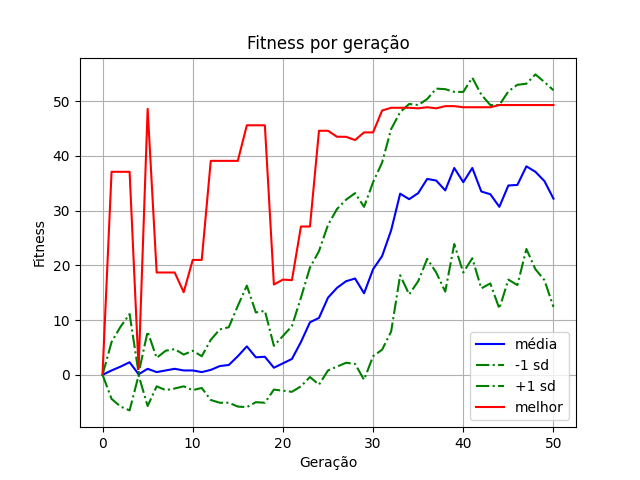
\includegraphics[width=0.8\textwidth]{imgs/deap_primeiro_algoritmo/fitness.png}
    \caption{Desempenho do primeiro algoritmo com base no fitness por geração.}
    \label{fig:primeiro_fitness_gens}
\end{figure}

\begin{figure}[!htbp]
  \centering
  \begin{subfigure}[b]{0.48\textwidth}
    \centering
    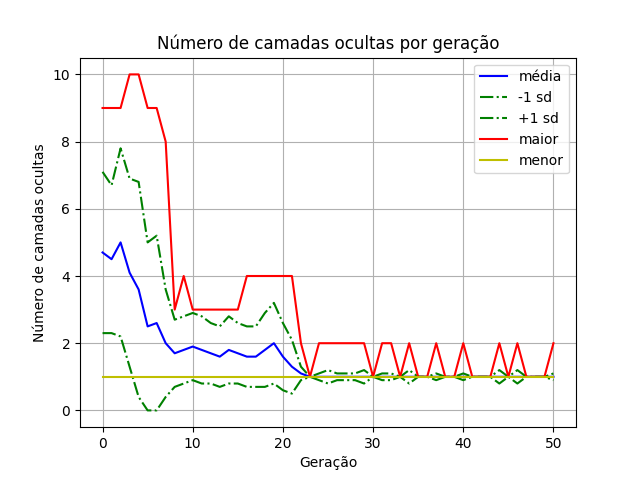
\includegraphics[width=\linewidth]{imgs/deap_primeiro_algoritmo/num_layers.png}
    \caption{Evolução da quantidade de camadas ocultas}
    \label{fig:sub1}
  \end{subfigure}
  % \hfill
  \begin{subfigure}[b]{0.48\textwidth}
    \centering
    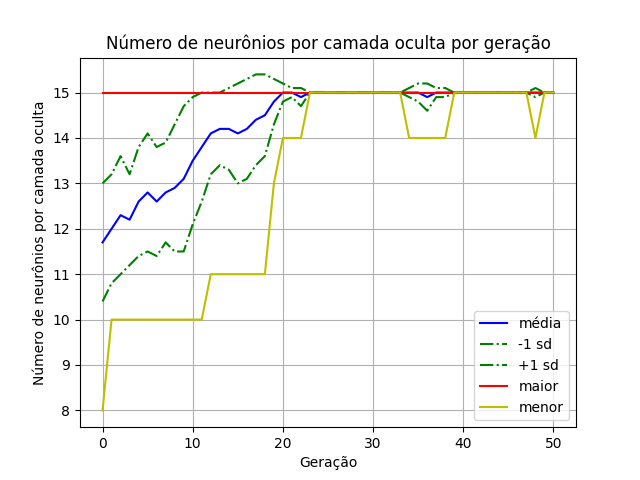
\includegraphics[width=\linewidth]{imgs/deap_primeiro_algoritmo/neurons.png}
    \caption{Evolução da quantidade de neurônios por camada oculta}
    \label{fig:sub2}
  \end{subfigure}
  \caption{Evolução da topologia da rede utilizando o primeiro algoritmo.}
  \label{fig:primeiro_topologia}
\end{figure}

\subsection{Utilizando DEAP - Coevolução}
Na Figura~\ref{fig:fitness_gens} pode ser observada a evolução do fitness desse algoritmo coevolucionário (evoluindo separadamente a topologia da rede e os pesos sinápticos), que encontrou o melhor fitness de \num{58,2} e média de \num{34,9}. O algoritmo foi executado de forma que cada população tenha \num{500} indivíduos e \num{100} macro-gerações, que por sua vez se dividem em \num{3} micro-gerações de evolução da topologia e \num{3} micro-gerações de evolução dos pesos sinápticos. Também foi implementado o processo de elitismo, no qual \num{10}\% dos melhores pais necessariamente continuam para a próxima geração. 

\begin{figure}[htbp]
    \centering
    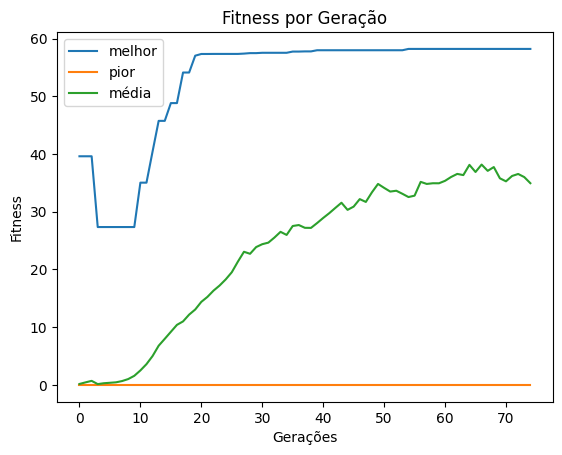
\includegraphics[width=0.8\textwidth]{imgs/fitness_gens.png}
    \caption{Desempenho do algoritmo com base no fitness por geração.}
    \label{fig:fitness_gens}
\end{figure}

\subsection{Utilizando NEAT}
Por fazer uma implementação nova de rede neural, o algoritmo com o NEAT foi mais rápido de rodar, já que não usa a biblioteca \textit{keras} e nem a \textit{pytorch} que adicionam \textit{overhead} na execução do algoritmo. Com isso, foi possível uma maior exploração de hiperpârametros e um tamanho maior da população.

Assim, o algoritmo foi executado com o tamanho da população de 1500 indivíduos, as opções de função de ativação foram \textit{sigmoid, relu} ou \textit{tanh}.

Na Figura~\ref{fig:neat_fitness_gens} é possível ver a evolução do fitness ao longo das gerações encontrando fitness máximo de \num{98,49}, ou seja, o drone conseguiu chegar e parar na localização alvo com o único ponto de melhoria sendo o tempo para alcançar o resultado, mas já muito próximo do fitness teórico máximo (\num{100}). A Figura~\ref{fig:neat_fitness_gens_começo} representa a mesma visualização, mas mostrando apenas as primeiras 100 gerações. Com isso, pode-se verificar que acontece uma grande evolução até por volta da geração 20, e depois o algoritmo necessita de mutações esporádicas para alcançar fitness melhores.
\begin{figure}[htbp]
    \centering
    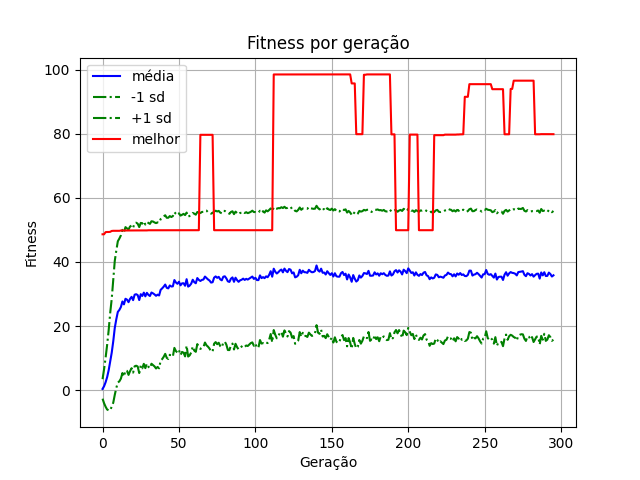
\includegraphics[width=0.8\textwidth]{imgs/neat/fitness.png}
    \caption{Desempenho do algoritmo NEAT com base no fitness por geração.}
    \label{fig:neat_fitness_gens}
\end{figure}
\begin{figure}
    \centering
    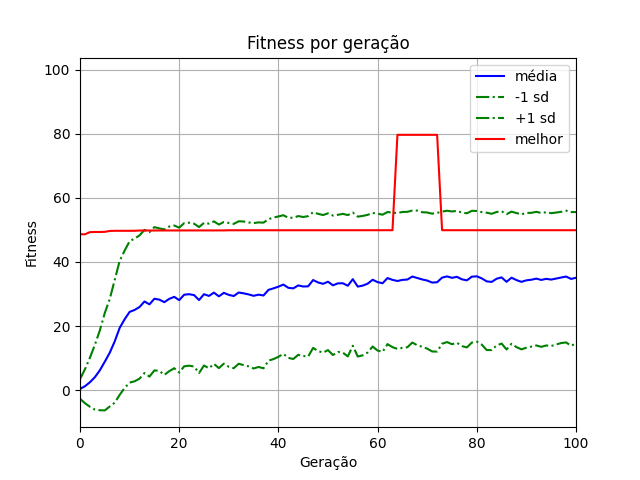
\includegraphics[width=0.8\textwidth]{imgs/neat/fitness_começo.png}
    \caption{Evolução de fitness do algoritmo NEAT nas primeiras 100 gerações.}
    \label{fig:neat_fitness_gens_começo}
\end{figure}


Na Figura~\ref{fig:neat_especiacao} é possível visualizar como ocorreu o processo de especiação na população. Sendo que a Figura~\ref{fig:species} demonstra o tamanho das espécies, ou seja, a quantidade máxima, mínima e média de organismos por espécie ao longo da evolução, enquanto a Figura~\ref{fig:number_species} demonstra a quantidade de espécies a cada geração. 

\begin{figure}[!htbp]
  \centering
  \begin{subfigure}[b]{0.48\textwidth}
    \centering
    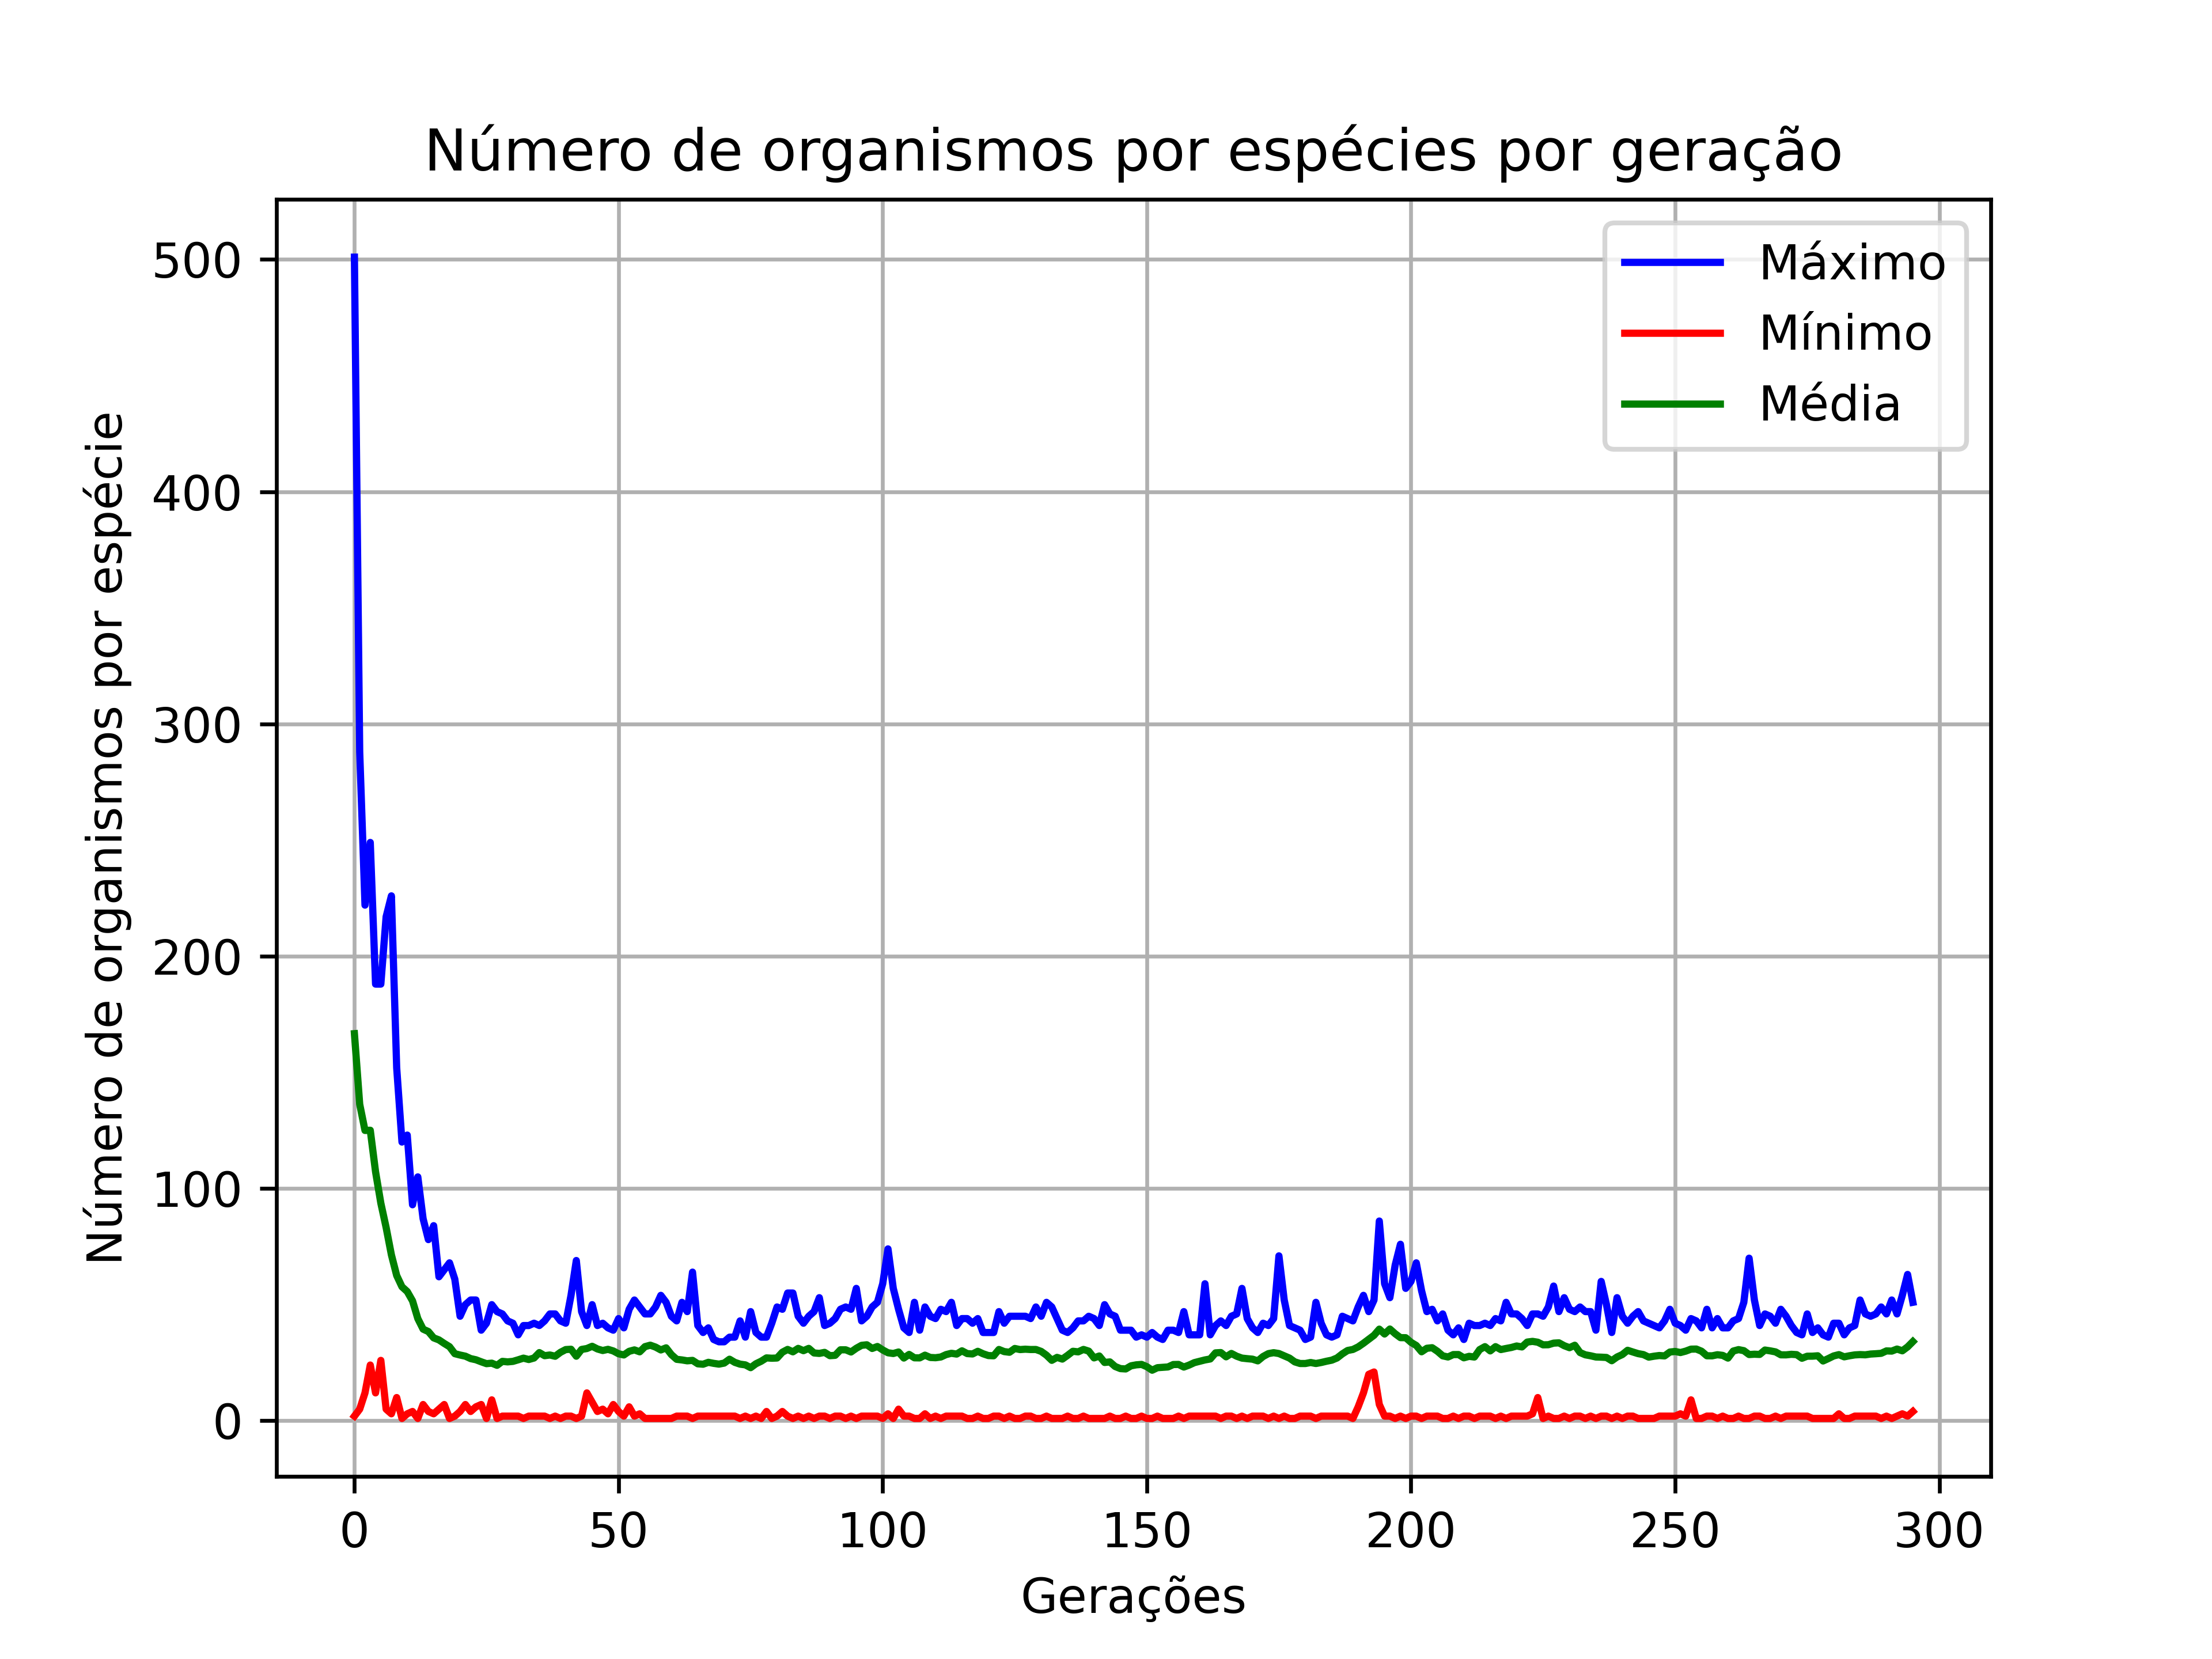
\includegraphics[width=\linewidth]{imgs/neat/size_species.png}
    \caption{Tamanho das espécies por geração.}
    \label{fig:species}
  \end{subfigure}
  % \hfill
  \begin{subfigure}[b]{0.48\textwidth}
    \centering
    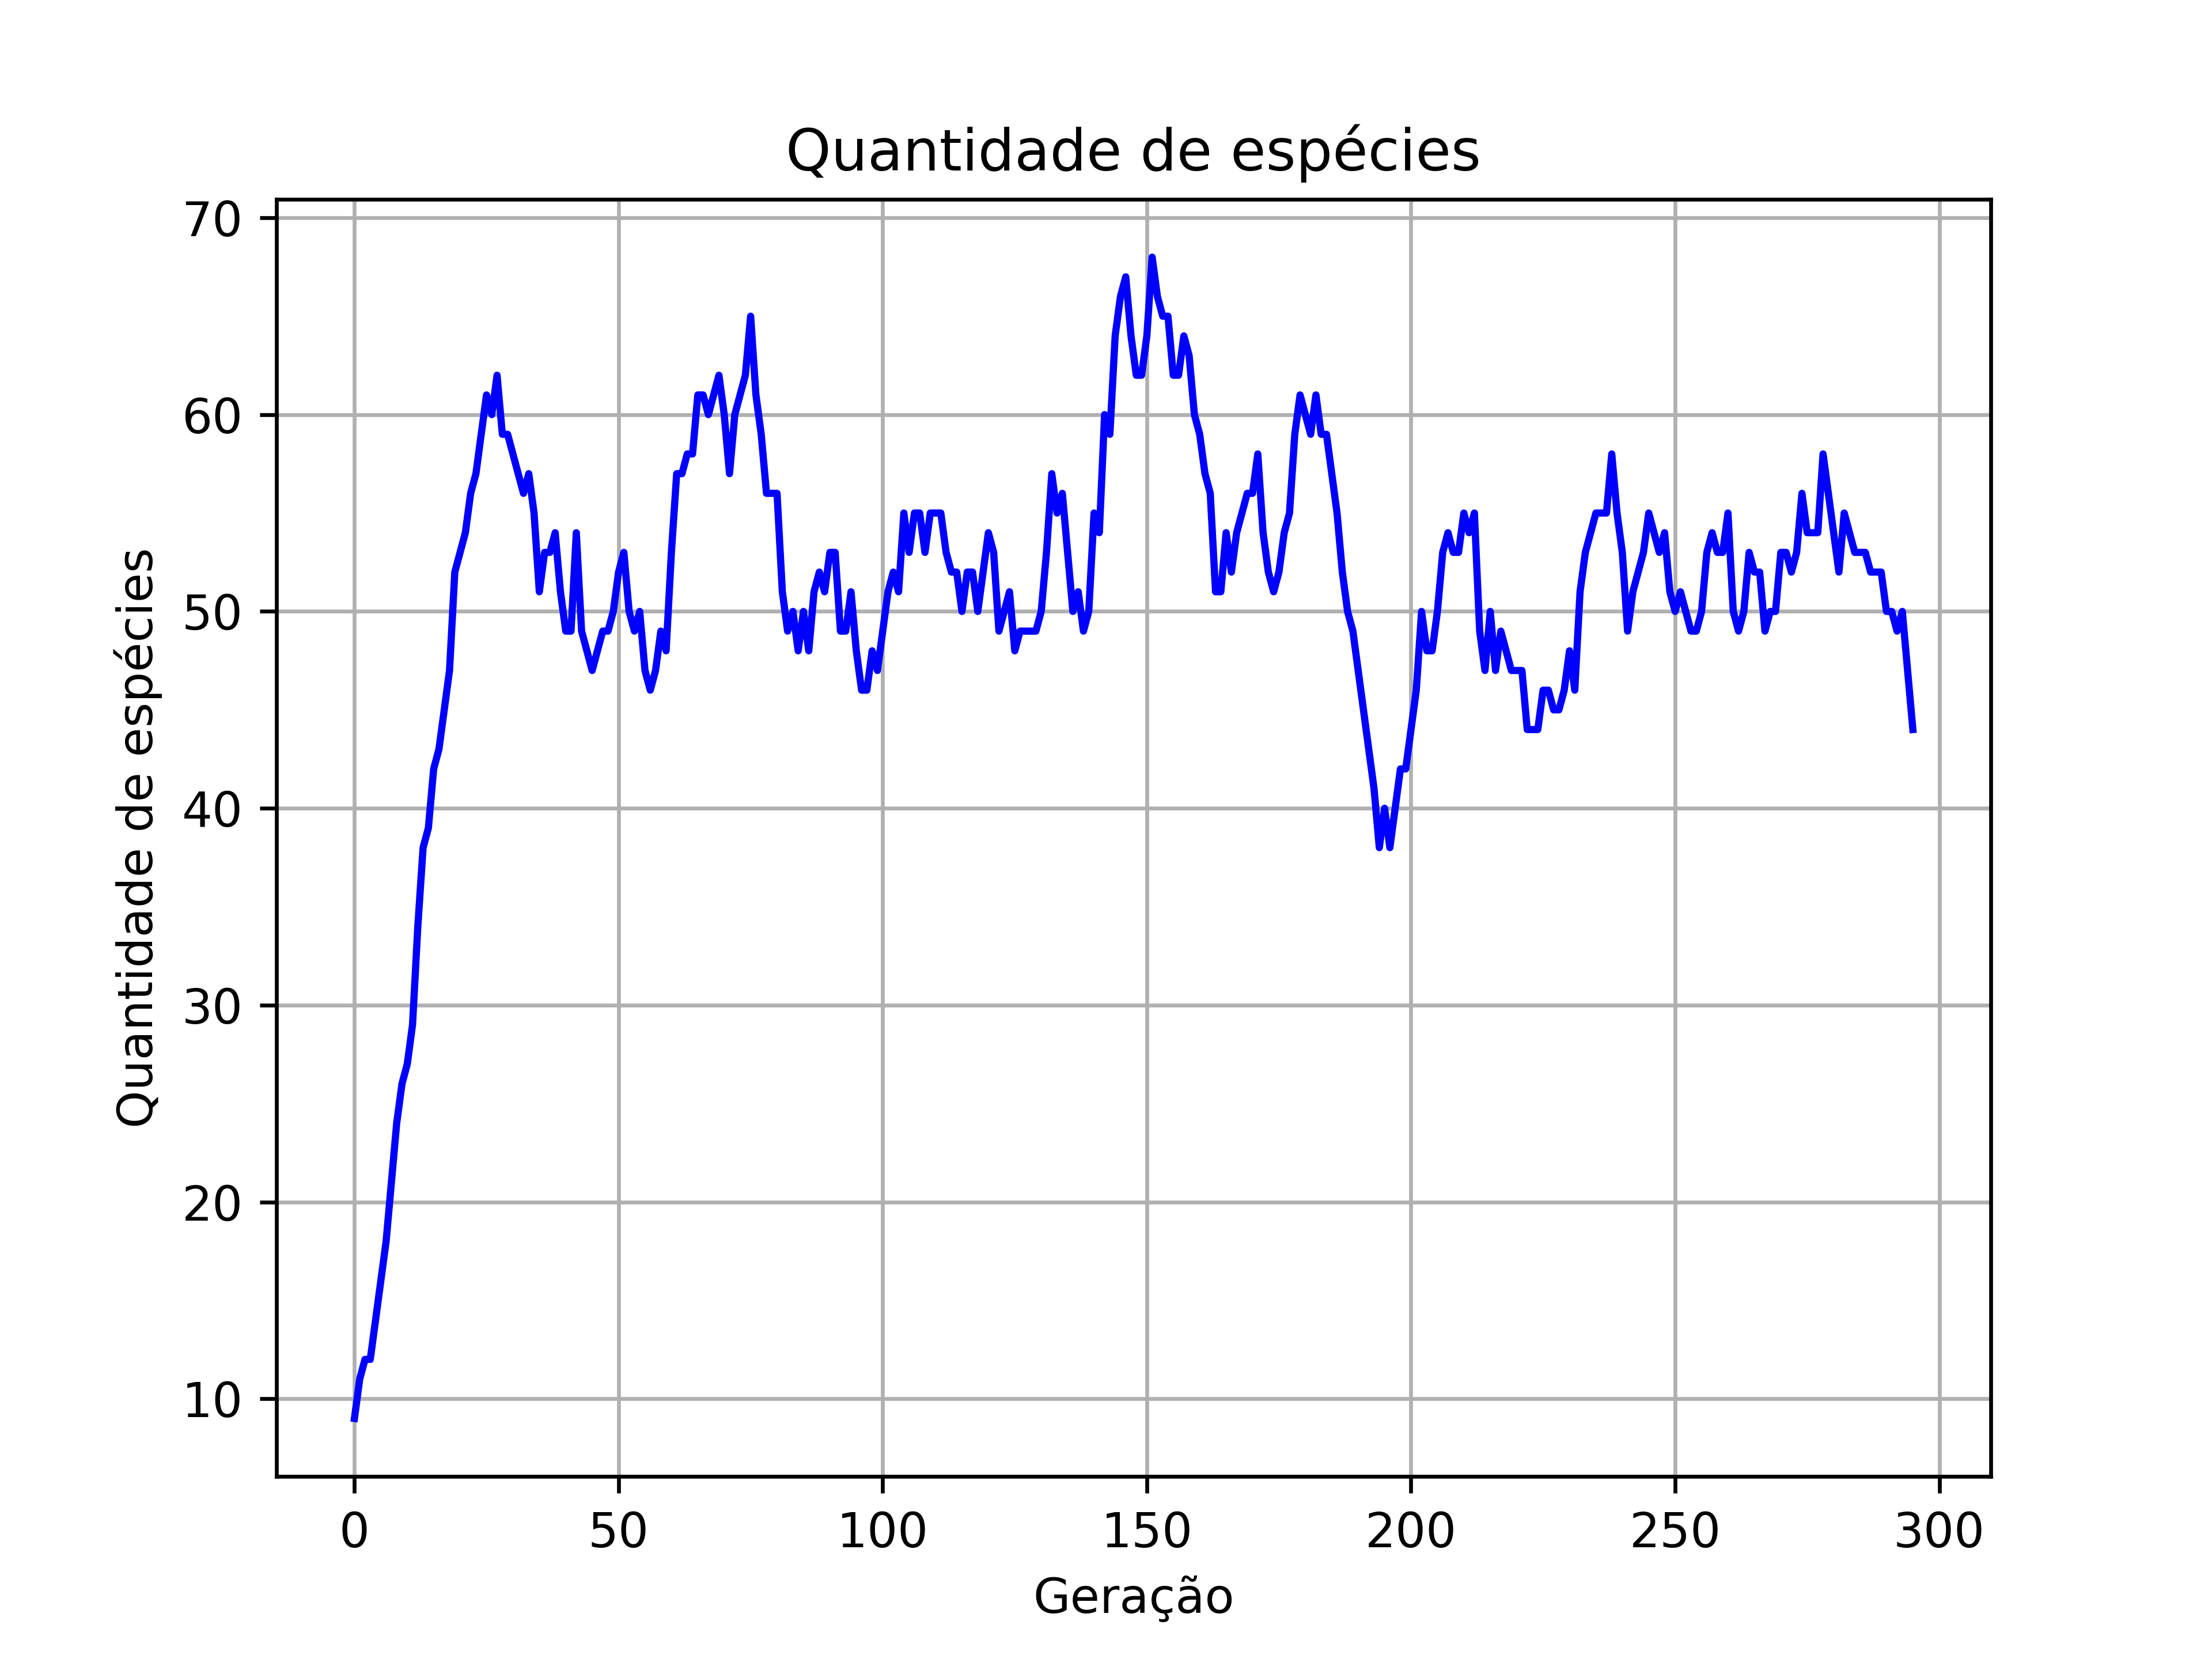
\includegraphics[width=\linewidth]{imgs/neat/number_species.png}
    \caption{Quantidade de espécies por geração.}
    \label{fig:number_species}
  \end{subfigure}
  \caption{Evolução da especiação da população.}
  \label{fig:neat_especiacao}
\end{figure}

Por fim, na Figura~\ref{fig:winner_net} é demonstrada a rede que teve o maior fitness, sendo que os nós com forma quadrada representam neurônios de entrada, já os nós redondos com índices de \num{0} a \num{3} são nós de entrada e, finalmente, os nós redondos remanescentes são neurônios de camadas intermediárias. As conexões de cor verde representam pesos positivos, enquanto as de cor vermelha representam pesos negativos. Ainda sobre as conexões entre nós, as tracejadas representam conexões desabilitadas. Portanto, é possível ver que a rede neural vencedora (com o maior fitness) teve dois neurônios intermediários com função de ativação \textit{relu}.
\begin{figure}[!htbp]
    \centering
    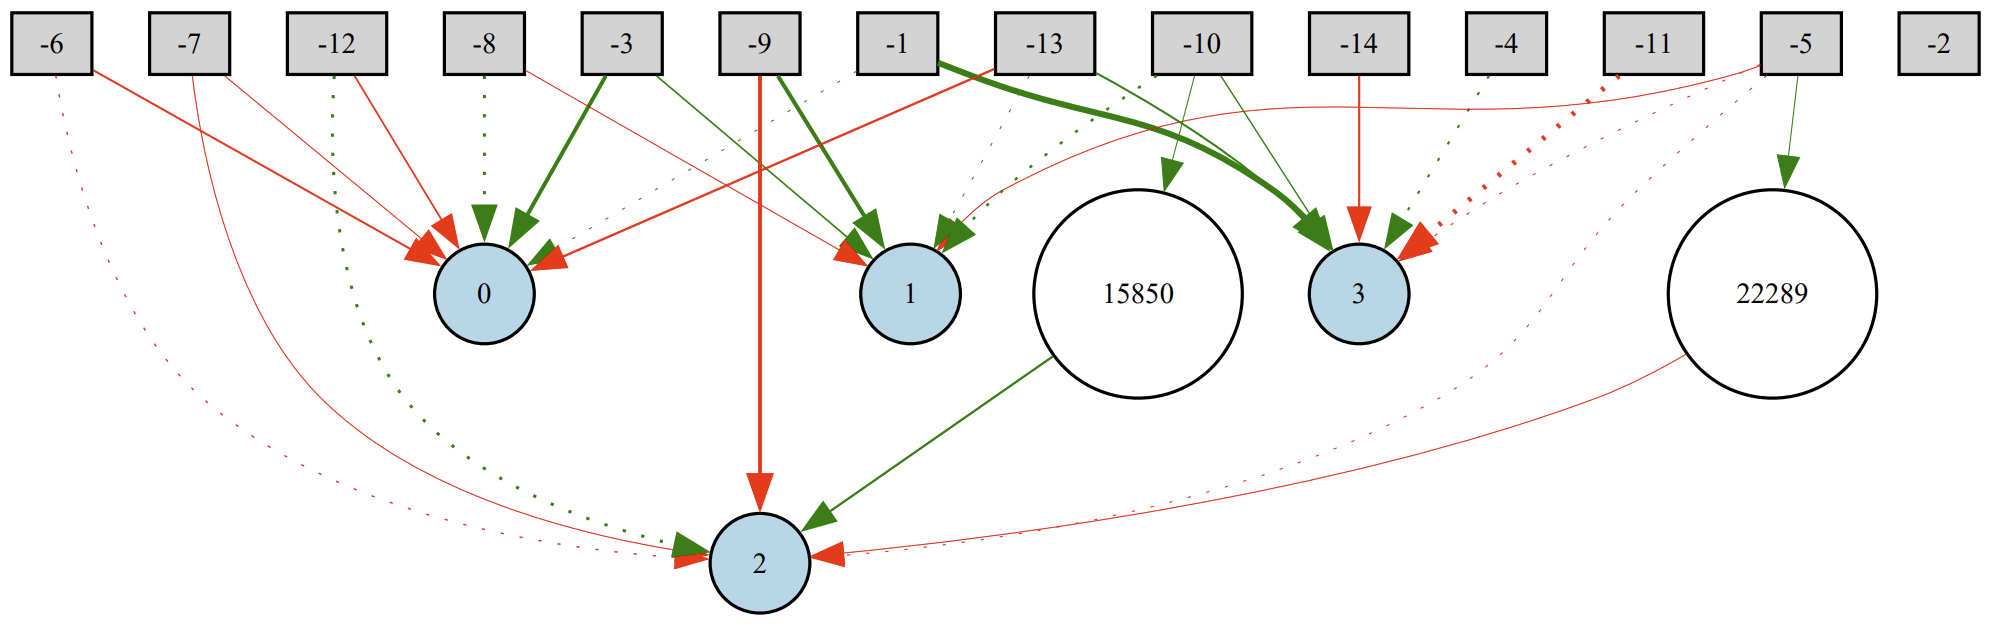
\includegraphics[width=0.8\textwidth]{imgs/neat/winner_net.png}
    \caption{Arquitetura da rede neural vencedora gerada pelo algoritmo NEAT.}
    \label{fig:winner_net}
\end{figure}

\section{Cronograma}
\begin{flushleft}
\begin{small}
\begin{tabular}{ |p{2.8cm}| *{12}{w{c}{0.59cm}|} }
 \hline
 \multirow{2}{2.8cm}{Etapas} & \multicolumn{7}{c|}{2024} & \multicolumn{5}{c|}{2025}\\
 \cline{2-13}
 &Jun&Jul&Ago&Set&Out&Nov&Dez&Jan&Fev&Mar&Abr&Mai \\
 \hline
 Revisão \newline Bibliográfica&\multirow{2}{0.59cm}{\centering \Huge \sffamily X}&\multirow{2}{0.59cm}{\centering \Huge \sffamily X}&\multirow{2}{0.59cm}{\centering \Huge \sffamily X}&\multirow{2}{0.59cm}{\centering \Huge \sffamily X}&\multirow{2}{0.59cm}{\centering \Huge \sffamily X}& & & & & & & \\
 \hline
 Desenvolvimento da Metodologia& &\multirow{2}{0.59cm}{\centering \Huge \sffamily X}&\multirow{2}{0.59cm}{\centering \Huge \sffamily X}&\multirow{2}{0.59cm}{\centering \Huge \sffamily X}& & & & & & & &\\
 \hline
 Implementação do Ambiente&&&&\multirow{2}{0.59cm}{\centering \Huge \sffamily X}&\multirow{2}{0.59cm}{\centering \Huge \sffamily X}&\multirow{2}{0.59cm}{\centering \Huge \sffamily X}&\multirow{2}{0.59cm}{\centering \Huge \sffamily X}&&&&&\\
 \hline
Implementação dos Algoritmos&&&&\multirow{2}{0.59cm}{\centering \Huge \sffamily X}&\multirow{2}{0.59cm}{\centering \Huge \sffamily X}&\multirow{2}{0.59cm}{\centering \Huge \sffamily X}&\multirow{2}{0.59cm}{\centering \Huge \sffamily X}&\multirow{2}{0.59cm}{\centering \Huge \sffamily X}&&&&\\
 \hline
 Análise dos \newline Resultados&&&&&&&&\multirow{2}{0.59cm}{\centering \Huge \sffamily X}&\multirow{2}{0.59cm}{\centering \Huge \sffamily X}&&&\\
 \hline
 Redação do \newline Relatório Final&&&&&&&&&\multirow{2}{0.59cm}{\centering \Huge \sffamily X}&\multirow{2}{0.59cm}{\centering \Huge \sffamily X}&\multirow{2}{0.59cm}{\centering \Huge \sffamily X}&	\\
 \hline
 Revisão e \newline Ajustes&&&&&&&&&&&&\multirow{2}{0.59cm}{\centering \Huge \sffamily X}\\
 \hline
\end{tabular}
\end{small}
\end{flushleft}

\bibliography{bibliografia}

\end{document}

